% Chapter Template

\chapter{Testing and Evaluation} % Main chapter title

\label{Chapter6} % Change X to a consecutive number; for referencing this chapter elsewhere, use \ref{ChapterX}

\lhead{Chapter 6. \emph{Testing and Evaluation}} % Change X to a consecutive number; this is for the header on each page - perhaps a shortened title

%----------------------------------------------------------------------------------------
\section{Introduction}

This chapter will focus on the testing and evaluation of the solution implemented. In order to evaluate how suitable the solution is at fulfilling the requirements, user based assessments were performed to collect feedback.

\section{Testing}

Before the assessments could begin, the application needed to be tested thoroughly so that the it would perform correctly and the feedback from the assessments would be most valuable. The testing was split into two sections, unit testing and functional testing.

\subsection{Unit Testing}

Unit testing is a form of automated software testing that individual executes portions of the code and validates whether the output is desirable or not. Unit testing is very useful in iterative based development where testing needs to be repeated often to ensure older features do not get broken by newer ones. This is a common issue in software programming, especially when many developers are working on the same code base and don't fully understand the entirety of it, resulting in undesirable changes and side effects commonly occurring.

Although some unit tests were written for this project using the 'Visual Studio Unit Testing Framework', I decided that the time cost for implementing the tests was not worth the output, especially as the project had a fairly small code base and I was the sole developer. Most of the features were also created independently of each other, resulting in a smaller risk of them modifying each others functionality.

\subsection{Functional Testing}

Functional testing is a requirement in any software development project to ensure it is ready for release. Functional testing is the manual act of testing the functionality of an application, just like an end user would. This helps to  identify functions of the application that are broken or poorly designed, ensuring that these functions do not make it to the end user.

\subsubsection{Testing Methodology}

In order to test the app's functions, an initial regression test was used. Regression testing is a form of functional software testing that seeks to uncover software bugs within certain features of a software application. An initial regression test includes all features implemented in the prototype. As extra features are added at a later date, new regression tests must be made for these features. Only once all features are tested and pass can the application be signed off for release.

To start regression testing, an extensive list of all the app's features was made. This test list comprised of the following information:

\begin{itemize}
	\item Test Number - A unique number for easily identifying the test.
	\item Feature Category - The category that the feature belongs to.
	\item Feature Type - The type of feature it is.
	\item Action - A description of feature and its desired effect.
	\item Pass/Fail - Whether the test was successful or not.
	\item Comments - Reason as to why the test failed or any improvements that could be made.
\end{itemize}

With the test list formulated, each feature was tested multiple times to determine if they should pass or fail by comparing the test action to the actual result.

\subsubsection{Results}

\begin{figure}[htbp]
	\centering
		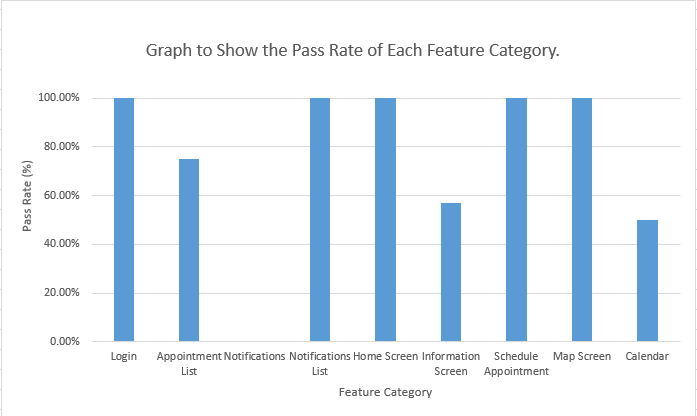
\includegraphics[width=\textwidth,height=\textheight,keepaspectratio]{Figures/FunctionalTestResults.png}
		\rule{35em}{0.5pt}
		\caption[Graph to show the pass rate of each feature category.]{Graph to show the pass rate of each feature category.}
	\label{fig:functionaltestresults}
\end{figure}

Appendix C shows the results of the initial regression test. The initial results showed that although the majority of the app was working as intended, the notification feature category was completely broken and needed fixed prior to the user based assessments.

\subsection{Further Testing}

Although aspects of the mobile application were fully tested, most of the testing was focused on the user interface and testing of the server was ignored. Further testing must be done to analyse how the system would perform in a production environment. Due the the system being a prototype, it was not necessary for this project.

\subsubsection{Load testing}

In order to assess how many concurrent users can successfully use the system before issues occur, load testing must be performed. This is a process where test accounts are created and accessed at the same time, which is repeated until performance  or other issues begin to occur. This helps to prepare for user demand and outline efficiency issues or the hardware requirements for the system prior to it being launched.

\subsubsection{Concurrency Issues}

One hypothetical issue came to mind when implementing the prototype; what happens when two separate users schedule the same appointment at the same time. Although the system is designed to be flexible enough such that these issues would not have a fatal effect on the system, it would likely create an error that is not currently handled by the client application. Many issues like this could exist, and features would have to be tested thoroughly to discover them all.

\subsection{Conclusion}

With the test results collected, any failures were investigated and the specific action was re-implemented. Final regression tests were repeated until all failures were passed and the prototype was ready for evaluation.

Further performance testing and analysis of the applications resource usage could also have been performed, but slow/poor performance was not picked up by the functional testing and was therefore deemed unnecessary.

%----------------------------------------------------------------------------------------

\section{Evaluation}

After testing was completed and the app was in a stable state, the evaluation could commence.

As stated in Section 2.5, I wanted to evaluate the solution based on the following questions:

\begin{itemize}
	\item How easy to use is the mobile application?
	\item Does the solution work? Does it fail occasionally?
	\item Is the solution missing key features?
	\item Would patients find the mobile application useful?
	\item Does the solution reduce wasted appointments?
	\item Does the solution reduce staff resources required for managing appointments?
	\item Does the solution increase the user experience when managing appointments?
\end{itemize}

In order to evaluate these questions, three methods of evaluation were proposed, user observation, user feedback and trials in real hospital environments.

\subsection{Evaluation of Methodology}

Whilst designing and implementing the prototype, it became apparent that the proposed solution was not ideal. Firstly, the solution could wrongly encourage patients to reschedule appointments when it is unnecessary. This would, without a doubt put strain on the system, making it hard for medical staff to constantly adapt to changes in the schedule.

This is however a hypothetical problem. When patients are faced with the probable long waiting times that they would in an hospital environment, it would be undesirable for them to reschedule appointments often. Trials of the proposed system would have to be run to determine whether the additional strain would exist or not.

Another problem the solution faces is that it would not be able to replace the current system entirely, as not all patients have access to smart devices and internet access. The system would have to be integrated alongside other systems in place, which could prove challenging with clinics that still use paper based approaches or rely on staff members for appointment management. As the number of patients without internet access is a growing minority, this may not be as problematic as first thought. Also, as the solution is designed to be platform independent, web interfaces could be set up in clinics and hospitals to accommodate for this, or even dedicated staff members to manage appointments through the system on a patient's behalf.

\subsection{Controlled Trials}

In order to evaluate the effects of the solution on staff resources and appointment wastage, trials would need to be carried out in real clinics and hospitals. This would produce statistical data that could then be compared with a control group who use the standard methods of appointment scheduling available today.

Unfortunately, it was not possible to conduct clinical trials for this project due to insufficient resources and the time restrictions involved. Despite this, I was able to conduct the user evaluation successfully and collected good feedback to evaluate the user experience of the application.

\subsection{User Observation}

User observation was carried out on a ten willing participants who were given a sheet with a list of tasks that they had to attempt (see Appendix E). Tasks were deliberately designed to be vague, not offering any instructions on how to complete a task. By designing the tasks this way, it demonstrated the applications usability and aimed to identify areas that were not intuitive.

Applicants were also provided with a test account with three hypothetical appointments already set up. The first two appointments were unscheduled to demonstrate the scheduling functionality of the app, and the third demonstrated the synchronisation with the phones calendar feature.

From observing the entire applicant group, none had issues completing all of the tasks given. Feedback was generally very positive for most of the features except the scheduling process. Some applicants showed signs of annoyance when trying to get the desired appointment which required a trial and error approach of inputting times and seeing if they were taken. Although the system offered a selection of choices close to the input time, this was not desirable for a user with a specific set of dates and times that they were available on.

Applicants also queried for a way to manage notifications, turning certain notifications on and off and highlighting a useful extension that could be added in the future.

\subsection{User Questionnaire}

The user questionnaire was designed (see Appendix F) to collect useful feedback and carried out after the user observation on the same participant group. The questionnaire consisted of numerical ratings of the mobile application and the following graph was composed from the average ratings provided from all ten applicants:

\begin{figure}[htbp]
	\centering
		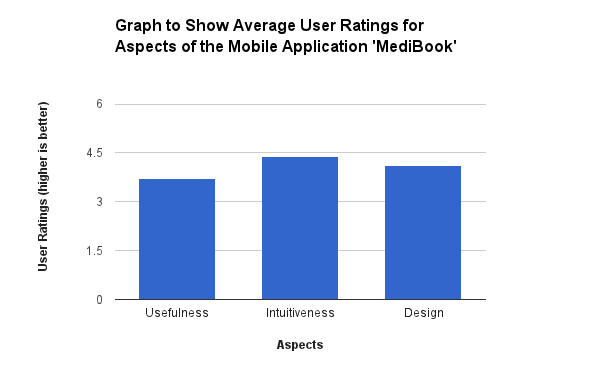
\includegraphics[width=\textwidth,height=\textheight,keepaspectratio]{Figures/AverageRatings.png}
		\rule{35em}{0.5pt}
		\caption[Graph to Show the Average User Ratings Collected from the User Questionnaire]{Graph to Show the Average User Ratings Collected from the User Questionnaire}
	\label{fig:questionnaireresults}
\end{figure}

The questionnaire also provided ways for the applicants to give feedback and suggestions. Some useful feedback included the suggestion of disabling unavailable times from the app's time picker fix the trial and error approach currently implemented. Some users also suggested possible future extensions such as using the notification feature for scheduling a patients medication, also providing them with prescription information and pharmacies located near the patient.

\subsection{Further Evaluation}

Besides the methods discussed above, many aspects are missing from the evaluation due to time restrictions and further evaluation could be performed in the future.

\subsubsection{Training}

Although the user evaluation showed that the app was intuitive, all participants admitted to owning their own smart device and had general knowledge on how to operate an Android application.

Further testing could be performed on a test group consisting of people who are not technically proficient. This would give a better analysis on training requirements and would help outline documentation and a manual for the applications operation.

\subsubsection{Comparison with Phone Appointment Booking}

As identified in the problem description, one of the main methods for booking a medical appointment currently is over the telephone, so further evaluation could be performed to identify the strengths and shortcomings of the prototype when compared with a telephone booking.

Participants would be asked to first book an appointment over the telephone, and then book the same appointment through the mobile application. They would then be interviewed on their findings. Some useful questions could be asked to compare the mobile app with telephone appointment bookings:

\begin{itemize}
	\item Is it faster to book via mobile?
	\item How many telephone staff members were required to fulfil demand?
	\item How many staff members were required to maintain the mobile application?
	\item Was more information available by telephone?
\end{itemize}

\subsection{conclusion}

Based on the findings obtained by the user evaluation, the prototype application can be judged as a success in terms of providing a good user experience. It is easy to use, did not fail during the user evaluation and participants found that it was useful. Although it was missing some features such as disabling unavailable times from the time picker, these could be implemented easily in the future.

However, although the user evaluation was successful, many other observations required for the evaluation of this system depend upon real world scenarios. More testing and evaluation of the system being used in real hospital and clinic environments would have to be executed before it could be deemed a success.

%----------------------------------------------------------------------------------------